\documentclass[
	12pt
] {article}

\usepackage[
	a4paper,
	left=1.5cm,
	right=1.5cm,
	top=2.5cm,
	bottom=2.5cm,
	headheight=1cm
] {geometry} %for setting margin

\usepackage{fancyhdr} %for header and footers
\usepackage{parskip} %for leaving some space after paragraphs


% Math
\usepackage{mathtools} %helps to number equations
\usepackage{siunitx} % Units of measurement


% For graphs and advanced diagrams
\usepackage{tikz} %the drawing library
\usetikzlibrary{positioning} %some auxilary to the drawing library
\usetikzlibrary{math} %helps to define variables in the tikz

\usepackage{authblk} %authors and their affiliations

% Basic graphics
\usepackage{float} %to force the figure to be in a place among the text
\usepackage{graphicx} %for include graphics
\usepackage{caption} %better referencing to labels
\usepackage{subcaption}  %helps with multiple pictures in a figure


% Language and Font package: COMMENT THESE FOR ENGLISH ONLY
\usepackage[T2A]{fontenc} %[RUS] loads cyrillic characters
\usepackage[russian]{babel} %[RUS] changes date heading 'abstract' to Russian
\usepackage[utf8]{inputenc} %[RUS] to force utf-8 encoding
\usepackage{hyperref}


%-----------------------------------------------------------------------

\renewcommand\thesubfigure{\asbuk{subfigure}} %[RUS] for renaming subfigures to russian
%\sisetup{output-decimal-marker = {,}} %[RUS] changes all ordinary decimal separator to rassiky commas
\pagestyle{fancy}
\graphicspath{{figures/}}


\newcommand\titleshort{Report}

\author[1]{Jamclub}

\affil[1]{Физтех-confessions}

\title{Физтех-сonfessions Report}
\fancyhead{}
\fancyhead[L]{Физтех-сonfessions}
\fancyhead[C]{\titleshort}
\fancyhead[R]{\the\year}


\sloppy
\begin{document}

\maketitle
\renewcommand{\arraystretch}{1.4}

\begin{abstract}
	Firstly, this report determines who is the most popular commentator of физтех-confessions, based on the number of likes each comment received.
	Secondly, compares the influence of the top few commentators with the rest of the audience.
	Thirdly, analyzes the number of posts and number of likes over time.
	If your name appears in this report and you think that you did not consent, then cry about it.
	\end{abstract}

\tableofcontents

\newpage
\section{Introduction}
\subsection{Definitions}
	\begin{enumerate}
		\item \textbf{active period:} when there is an active admin and there are regular posts, in contrast to depressions, when there is no admin, or no active admin.
		\item \textbf{audience:} the set of authors, writers, readers.
		\item \textbf{author:} the human who writes the comment.
		\item \textbf{density:} the number of likes per comment for a author.
		\item \textbf{hashtag:} a post of физтех-confessions, containing an unique hashtag number.
		\item \textbf{post:} a post on vk with a unique link, it can contain multiple hashtag-posts if it is a однострочки-post, for example: \#11202, \#11203, \#11204.
		\item \textbf{raw data:} unprocessed preliminary data.
		\item \textbf{table:} data which has headings, columns and rows.
		\item \textbf{writer:} the human who writes the post.
	\end{enumerate}
	
	
\subsection{Motivation}
	2024 was a great year! Физтех-confessions was used:
	\begin{enumerate}
		\item To confess love and sins
		\item As a means to procrastinate from doing work
		\item To pass depression
		\item To get daily dose of cringe because the brain demands it, just as our body demands \num{2.5}L of water everyday
		\item To share some brilliant memes.
	\end{enumerate}
	
	The audience would be glad to know who is the most popular author, and how the productivity of the writers has evolved over time.

\subsection{Source}
	\begin{table}[H]
		\centering
		\caption{Statistics on the raw data}
		\label{table:basic-stats-number-likes-comments-author}
		\begin{tabular}{| p{6cm}  c |}
			\hline
			Number of posts recorded: & \num{5000} \\
			\hline
			Total number of comments: & \num{17753} \\
			Total number of authors: & \num{1778} \\
			\hline
			Average number of comments per author: & \num{9.98} \\
			\hline
			Hashtag and date of the oldest post recorded: & \#4903 08.05.2023 \\
			Hashtag and date of the newest post recorded: & \#13312 11.12.2024 \\
			\hline
		\end{tabular}
	\end{table}
	
	An amateur code \cite{code-scrape-py} iterated through 5000 posts (\#4903 -- \#11312), and recorded the following:
	\begin{enumerate}
		\item Number of likes on each comment.
		\item The author of the comment.
		\item The number of likes on the post.
	\end{enumerate}
	
	The number of hashtags is not equal to the number of posts, $13312 - 4903 + 1 \neq 5000$, because:
	\begin{enumerate}
		\item Deleted posts, for example in \{\#2, \#3, \#10\}, actual number of posts = 3, number of hashtags based on the max and min, $10 - 2 + 1 = 9$.
		\item Однострочки and говнострочки.
		\item Possibly, a bug in the code which simply fails to read a page.
		\item Possibly, the code fails to read, because vk forces the code to login to view the page.
	\end{enumerate}
	The last two points are noted as possibility because the quantity of Однострочки was not measured, lets assume that an однострочки-post on average has 6 hashtags, and see if the numbers make sense.
	
	\begin{table}[H]
		\centering
		\caption{Possible proportion of однострочки-posts}
		\label{table:count-post-one-liners}
		\begin{tabular}{| c | p{6cm} | c |}
			\hline
			1 & Number of posts with single hashtag: & \num{4318} \\
			\hline
			2 & Number of однострочки-posts: & \num{682} \\
			3 & Average number of hashtags in one однострочки-post (assumption): & \num{6} \\
			\hline
			4 & Total posts (checking row 1 and 2): & $4318 + 682 = 5000$ \\
			\hline
			5 & Total hashtags (from row 1, 2, and 3): & $4318 + 6 * 682 = 8410$ \\
			6 & Total hashtags (actual, from recorded hashtags): & $13312 - 4903 + 1 = 8410$ \\
			\hline
			7 & Percent of однострочки-posts: & $682 / 5000 = \num{13.6}\%$ \\
			\hline
		\end{tabular}
	\end{table}
	
	Since all numbers in table \ref{table:count-post-one-liners} looks reasonable, we can assume that the possibility something was not read due to the fault of the code is low. The code was last used to make recordings on 11.12.2024, it might not be usable anymore because vk has made drastic changes in the html formatting of their website.

\subsection{Possible errors}
	The code could not read the less liked comments if the page of the post had a lot of comments. Because such comments are collapsed and the code was not smart enough to click on buttons and expand to read all comments. Since vk tends to hide the less popular comments by default, this created some inflation in the number of likes on comments. Since the sample size is still very large, such errors do not distort the conclusions on who is the best commentator.
	
	Vk.api would give correct data but it was not used due to task being too technically difficult in nature when the benefit is only slightly improved accuracy.
	
	\textbf{The raw data was not touched in anyway, extreme precaution was taken when it was copied from .txt output files to the google-sheet \cite{sheet-main}. If mistakes in calculations, wrong cell addresses or typos in the formulas are found, they are UNINTENTIONAL.}

\newpage
\section{Commentator}
\subsection{The most Liked commentator (count\_likes)}
	Definitions:
	\begin{itemize}
		\item count\_likes: the total number of likes an author received for the whole data.
		\item serial: the rank when the table is sorted based on count\_likes.
	\end{itemize}

	\begin{table}[H]
		\centering
		\caption{Top-20 authors with most likes \cite{sheet-count-likes}.}
		\label{table-count-likes}
		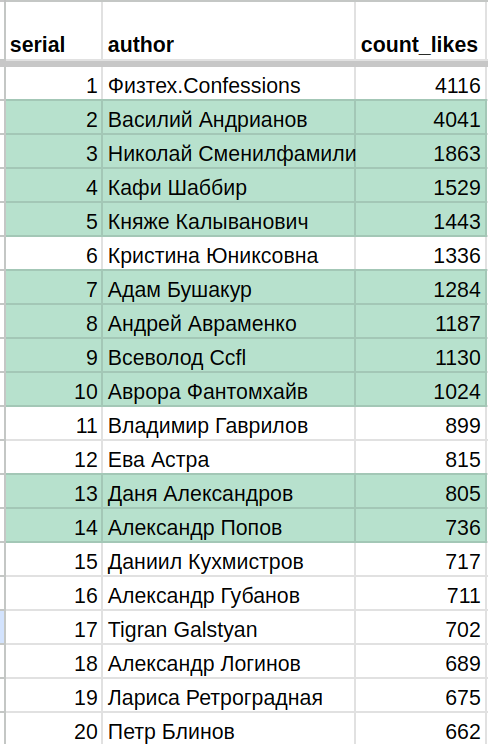
\includegraphics[width=0.5\textwidth]{table-count-likes-488}
	\end{table}

	Everyone is in the league of 1000's but \textbf{Василий Андрианов} is on another league collecting \num{4000} likes.

	\begin{table}[H]
		\centering
		\caption{Top-10 and top-40 authors' proportion of comments and likes, comparison.}
		\label{table:basic-stats-number-likes-comments-author}
		\begin{tabular}{| p{5cm} | c | c | c |} % or ccS
			\hline
			 & top-10 (green) & top-40 & all \\
			\hline
			count\_likes &
				\num{15042} \textbf{(\num{19.8}\%)} &
				\num{35536} \textbf{(\num{46.8}\%)} &
				\num{75881} \textbf{(\num{100}\%)} \\
			count\_comments &
				\num{2291} \textbf{(\num{12.9}\%)} &
				\num{7846} \textbf{(\num{44.2}\%)} &
				\num{17753} \textbf{(\num{100}\%)} \\
			density (likes per comment) &
				\num{6.57} &
				\num{4.5} &
				\num{4.27} \\
			\hline
		\end{tabular}
	\end{table}

	\begin{figure}[H]
		\centering
		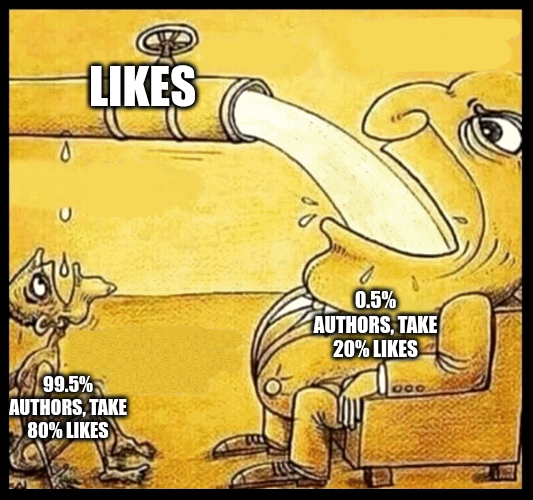
\includegraphics[width=0.5\textwidth]{fig-small-author-take-almost-all-likes}
		\caption{A few authors take a lot of likes}
		\label{fig-small-author-take-almost-all-likes}
	\end{figure}

	We can also say that half of the comment activity comes from just 40 authors. Now for simplicity, let us consider only the top-500 authors, and will have a look at the distribution curve on how the likes are distributed among these 500 authors. It is reasonable to take the top-500 instead of all \num{1778} because, the 500th author when sorted on count\_likes had only 18 likes in total. We can assume that 501st author and onward do not have much desire to get likes, therefore it will not be fair to add them to the distribution curve and conclude that the like distribution among the rich and poor is very large. By rich, of course we mean, those who took a large share of the total likes, and by poor who took a small share of the total likes. Also, the top-500 contribute to \num{93}\% of the total likes, so completely removing the others does not leave a big proportion of the data out.

	\begin{figure}[H]
		\centering
		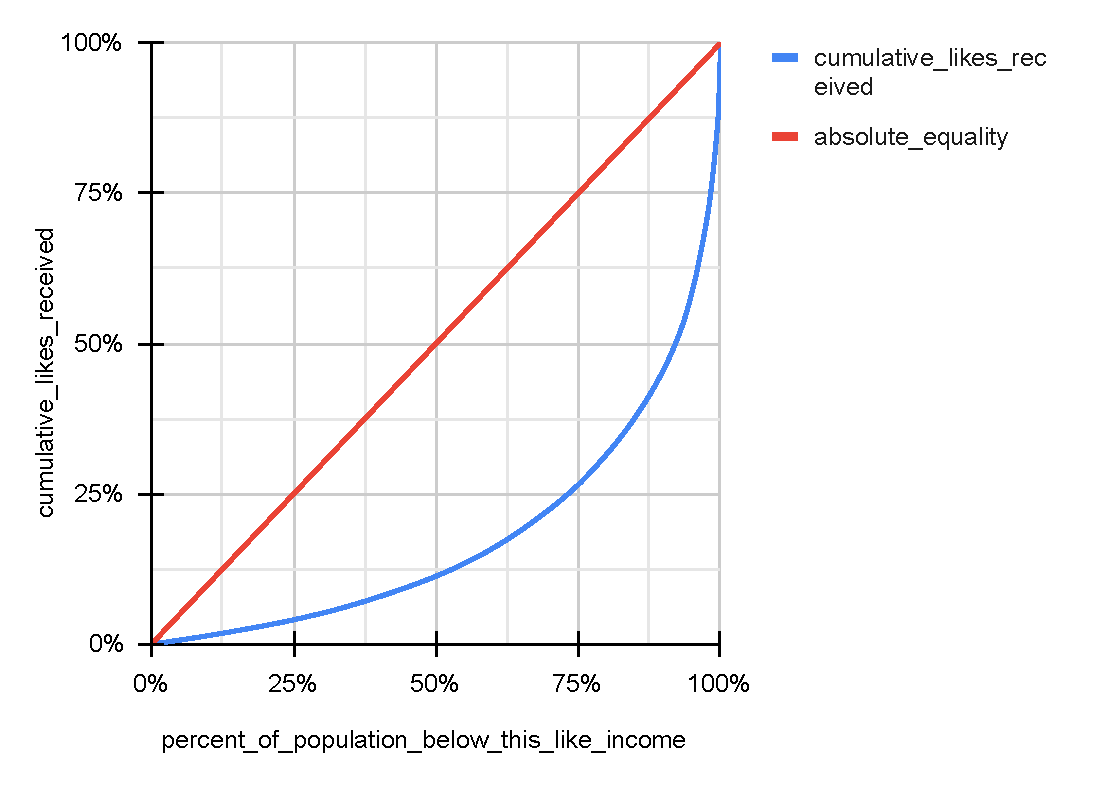
\includegraphics[width=0.8\textwidth]{fig-gini-calculation}
		\caption{Determination of gini-coefficient \cite{wikipedia-gini}, from the top-500 activity of top-500 authors \cite{sheet-calc-gini-coefficient}.}
		\label{fig-gini-calculation}
	\end{figure}

	Here, we can say that, the top-10 are the top \num{2}\% wealthy men and the top 40 are the top \num{8}\% wealthy men in физтех-confessions. Since $10/500 = 2\%$, and $40/500 = 10\%$, and wealth is the total number of likes received for all the comments that was analyzed. We see that the top-2\% and the top-8\% have taken \num{26.7}\% and \num{50.1}\% of the likes respectively.

	In figure \ref{fig-gini-calculation}, the gini coefficient is \num{0.64}. Which means our inequality is similar to South Africa. In other words in South Africa, the top-\num{2}\% richest men take \num{26.7}\% of the country's annual wealth, and the top-\num{8}\% of the the richest men takes \num{50.1}\% of the country's annual wealth, except in our case luckily it is not food, water and iron, but just the amount of adrenaline rush from receiving notifications of a comment being liked. For comparison, we can look at other countries:
	\begin{table}[H]
		\centering
		\caption{Gini-coefficients of various countries}
		\label{table:gini-countries}
		\begin{tabular}{| c | c | c |} % or ccS
			\hline
			rank & country & gini-coefficient \\
			\hline
			1 & South Africa & \num{0.65} \\
			2 & Физтех-confessions & \num{0.64} \\
			3 & USA & \num{0.39} \\
			4 & Russia & \num{0.36} \\
			5 & Sweden & \num{0.29} \\
			6 & Norway & \num{0.23} \\
			\hline
		\end{tabular}
	\end{table}

\subsection{The most Depressed commentator (count\_comments)}
	Definitions:
	\begin{itemize}
		\item \textbf{rank: position based on a characteristic for a local table,} while the serial is always the rank when the table was sorted according to count\_likes.
		\item count\_comments: the total number of comments an author wrote.
		\item sr-difference = serial - rank, is the difference between the the positions in the table of count\_likes and in this table. We would want to know if we change the measure based on which we sort the table how much do the positions differ from the table which was sorted based on count\_likes.
	\end{itemize}

	\begin{table}[H]
		\centering
		\caption{Top-20 authors with most comments, \cite{sheet-count-comments}.}
		\label{table-count-comments}
		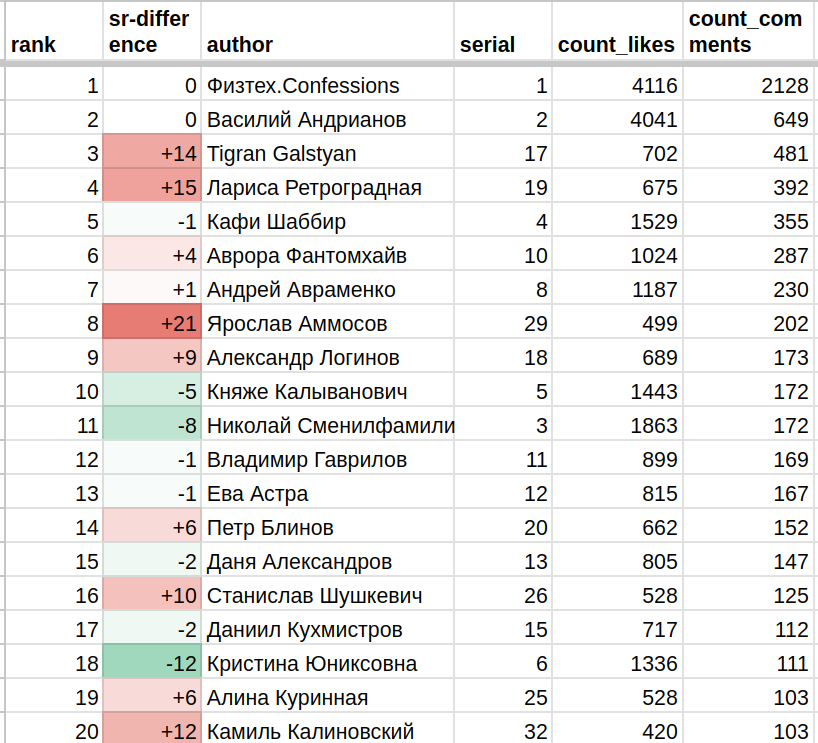
\includegraphics[width=0.7\textwidth]{table-count-comments-818}
	\end{table}

	Certainly the most depressed student in физтех writes the most amount of comments. And now by the legendary sr-difference we see that Tigran Galstyan has moved up 14 places as compared to Table \ref{table-count-likes}. Лариса Ретроградная has also moved up a massive amount of 15 places it is because her comments are self contradictory, trolling or just toxic. Ярослав Аммосов has moved up many places it is because his comments are usually emojis or compliments appreciating the post or a comment of another author. Кафи Шаббир has moved down one place which indicates that his ratio of quality over quantity if not neutral, slightly good for the community. \textbf{Николай Сменилфамилиюнавзрослуюсерьёзную has gone down by 8 places which means his quality over quantity is pretty high}.

	\begin{figure}[H]
		\centering
		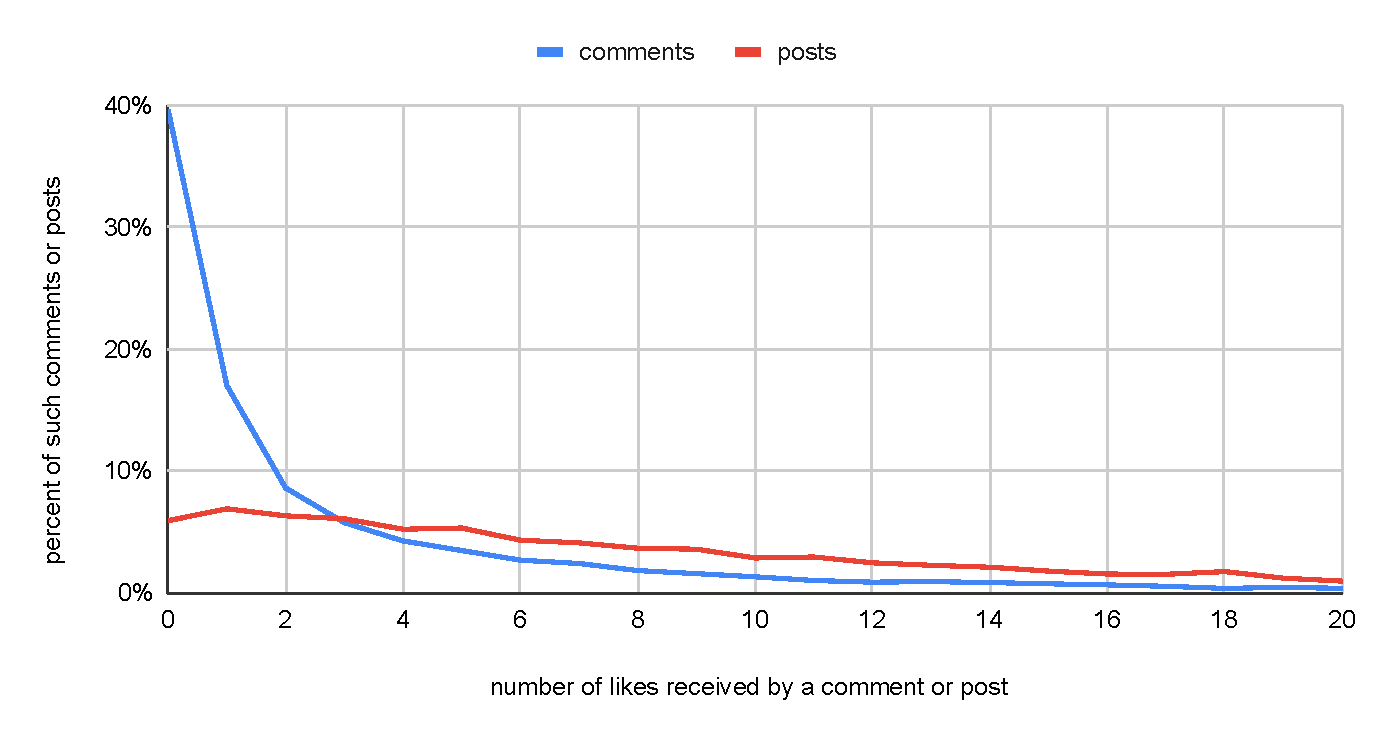
\includegraphics[width=1\textwidth]{fig-proportion-of-posts-or-comments-with-certain-likes}
		\caption{Percent of comments or posts which has the given number of likes.}
		\label{fig-proportion-of-posts-or-comments-with-certain-likes}
	\end{figure}
	Now let us see how the likes on comments are distributed. In other words what percent of comments have 0 likes and what percent of comment have more than 5 likes. In figure \ref{fig-proportion-of-posts-or-comments-with-certain-likes}, if you read for the blue curve $(x, y) = (2, 10\%)$, it means that \num{10}\% of the comments have \num{2} likes. The red curve is the like distribution for the posts on confessions. As expected the curve for the posts decreases smoothly and maintains a large enough positive value for $\num{20} + $ likes, but for comments $\num{40}\%$ of the comments have 0 likes and the proportion of comments as the number of likes increases falls much more rapidly than that of физтех-confessions posts.

	\begin{figure}[H]
		\centering
		\begin{subfigure}[b]{0.49\textwidth}
			\centering
			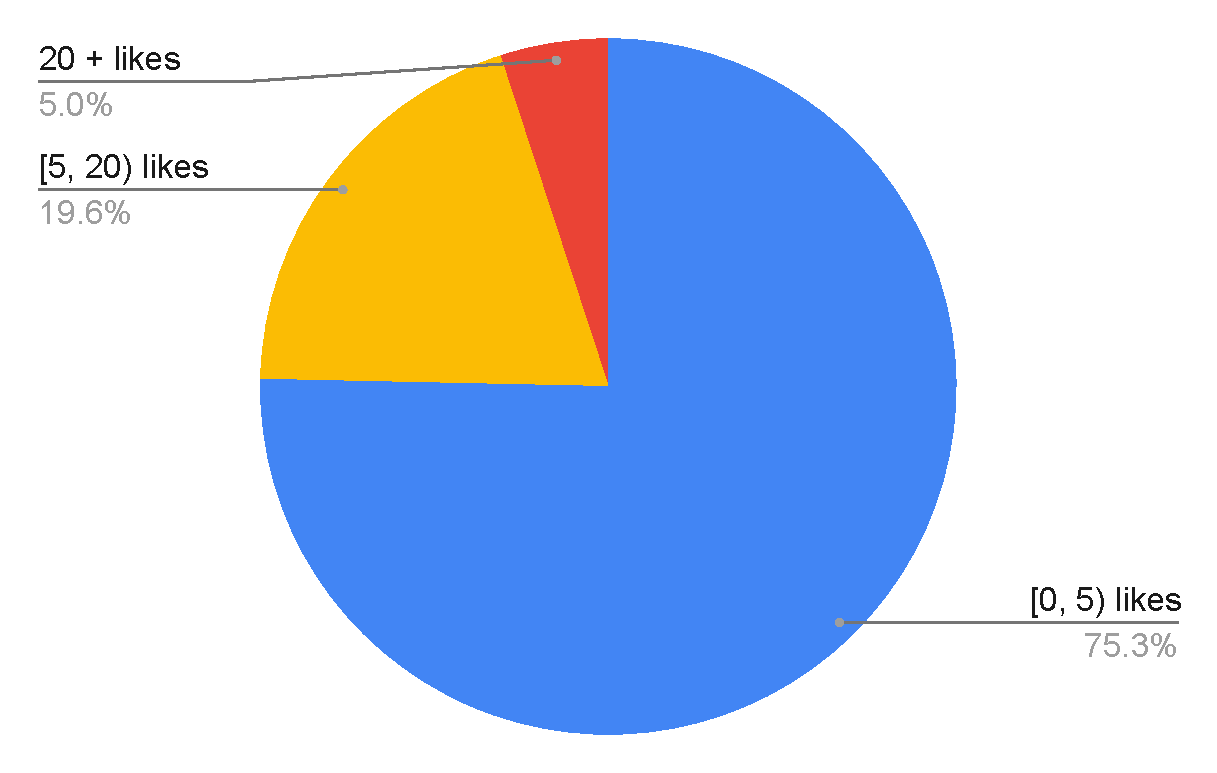
\includegraphics[width=\textwidth]{fig-proportion-of-comments-by-likes}
			\caption{Comments}
		\end{subfigure}
		\hfill
		\begin{subfigure}[b]{0.49\textwidth}
			\centering
			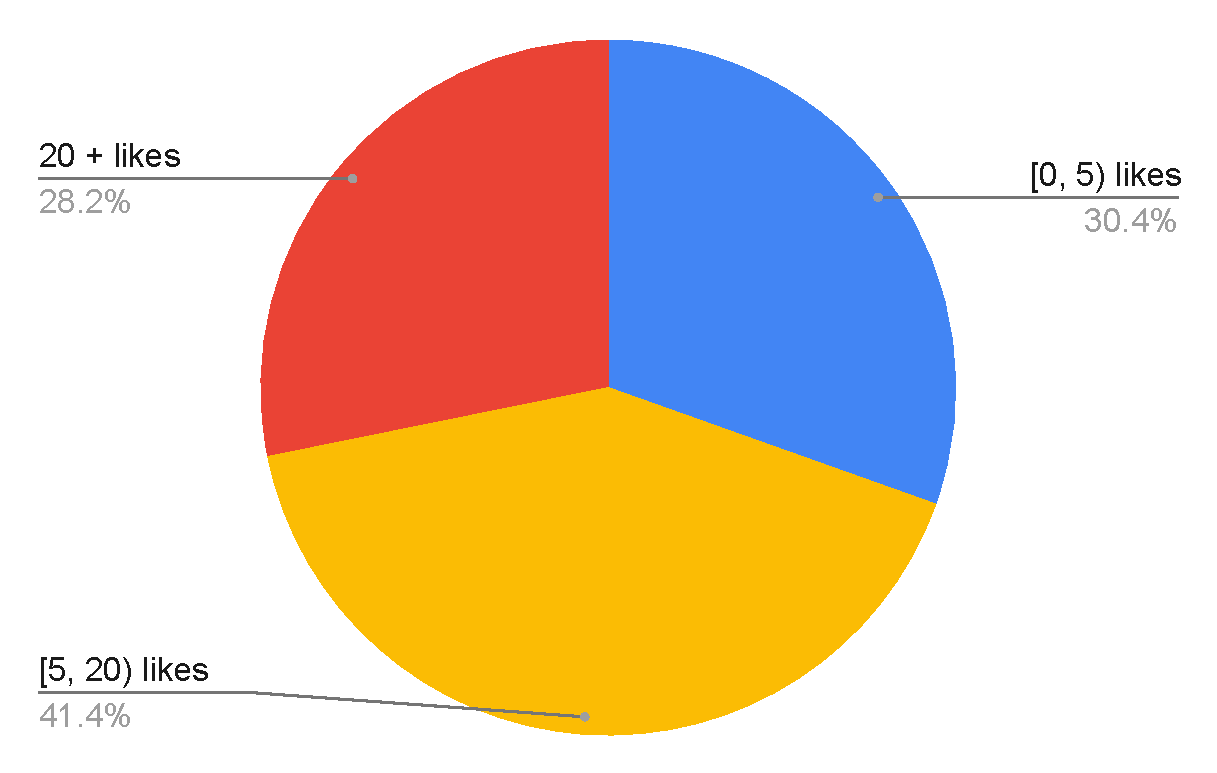
\includegraphics[width=\textwidth]{fig-proportion-of-posts-by-likes}
			\caption{Posts}
		\end{subfigure}
		\caption{Proportion of likes for comments and posts.}
		\label{fig-proportion-of-comments-or-posts-by-likes}
	\end{figure}

	In figure \ref{fig-proportion-of-comments-or-posts-by-likes}, we see that only \num{5}\% of the comments have more than \num{20} likes while, \num{28.2}\% of the posts have more than \num{20} likes.

\subsection{The most Sigma commentator (density)}
	\begin{table}[H]
		\centering
		\caption{Top-30 authors sorted according to density \cite{sheet-density}}
		\label{table-density}
		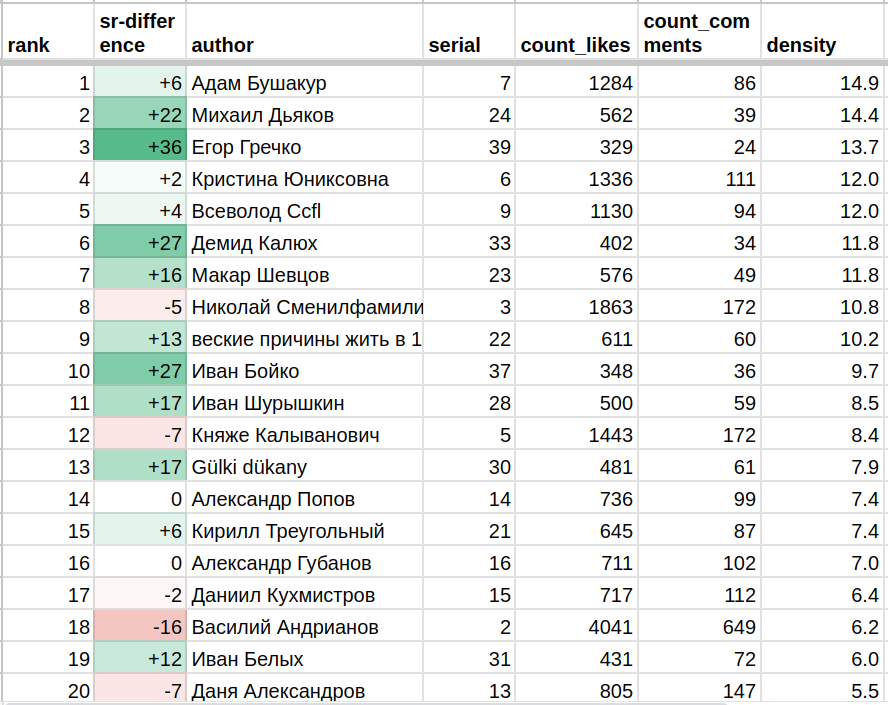
\includegraphics[width=0.75\textwidth]{table-density}
	\end{table}

	The number of likes and the number of comments certainly does not give us all the information. These are sigma's who keep silent, but when they speak something, it caries a lot of value. Кафи Шаббир completely flew away form the list ending up at 30th place. \textbf{Адам Бушакур is certainly the sigma here, his density given the amount of comments he wrote can be matched by a few}.

	\begin{figure}[H]
		\centering
		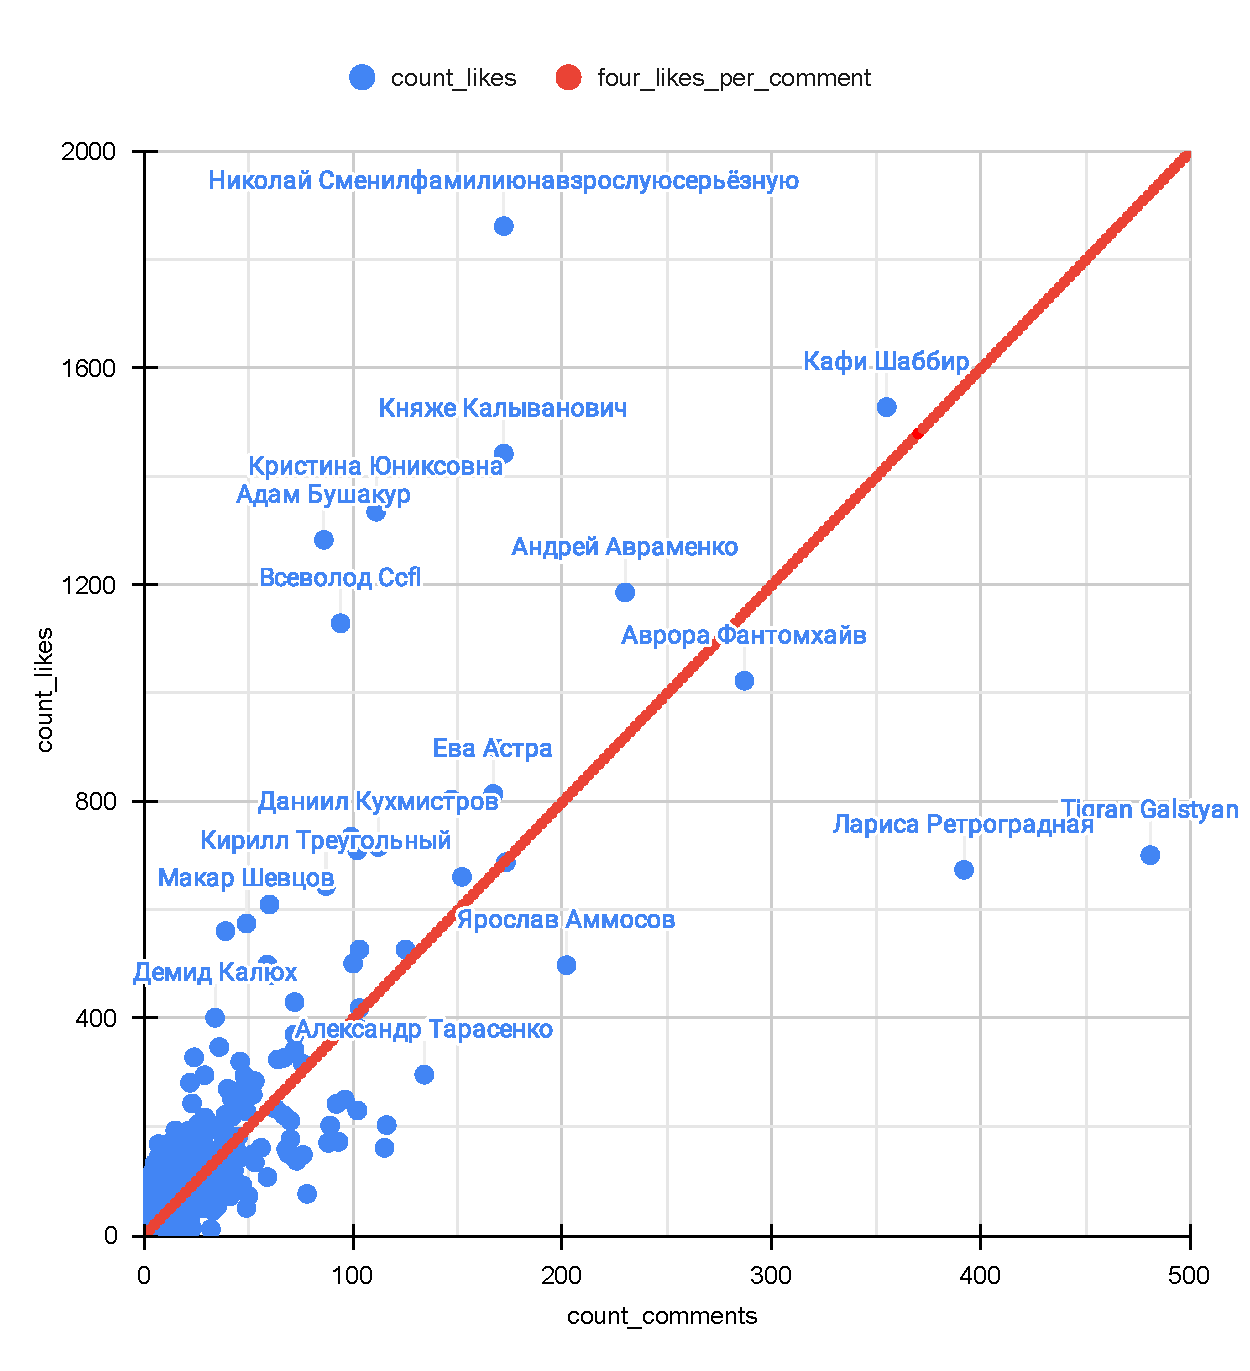
\includegraphics[width=0.7\textwidth]{fig-count-likes-comments-author-points}
		\caption{Number of likes vs comments for different authors, as points on a graph.}
		\label{fig-count-likes-comments-author-points}
	\end{figure}


	In figure \ref{fig-count-likes-comments-author-points} we can draw a line called the line of four\_likes\_per\_comment, this line represents the average density of all comments of all authors. Here Физтех.Confessions and Василий Андрианов were excluded to keep the scales of axes reasonable. Кафи Шаббир just managed to keep himself above this line while Аврора Фантомхайв is close to this line but below it. Now based on this line we can place our beloved authors into 4 zones.

	\begin{figure}[H]
		\centering
		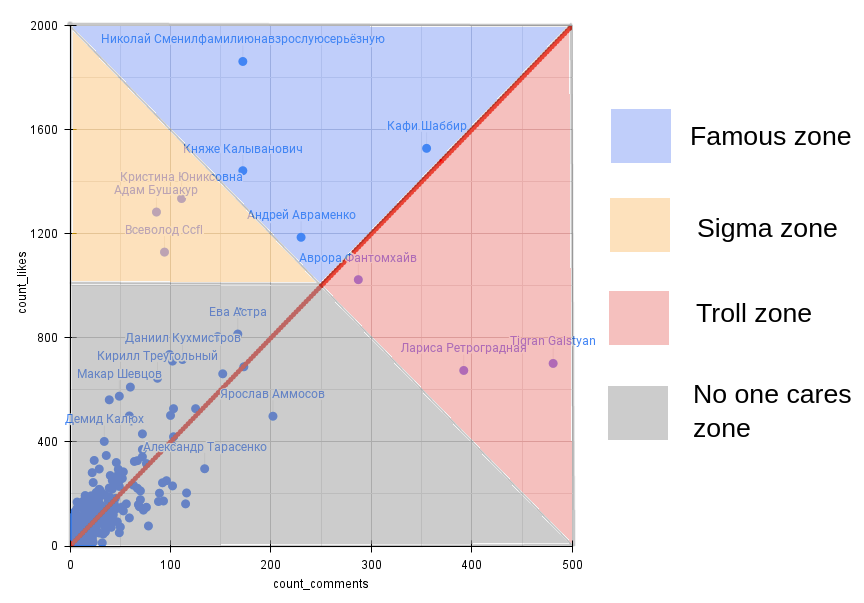
\includegraphics[width=0.9\textwidth]{fig-likes-vs-comments-divided-into-zones}
		\caption{The four zones on likes vs comments plot of various authors.}
		\label{fig-likes-vs-comments-divided-into-zones}
	\end{figure}

	\begin{enumerate}
		\item \textbf{Famous zone}: most of the audience will recognize the name of these authors.
		\item \textbf{Sigma zone}: not everyone know them, but those who know the author, immensely value what the author writes.
		\item \textbf{Troll zone}: their troll and toxic comments are often a cancer to the eye.
		\item \textbf{No one cares zone}: a small number of people know them or care about them.
	\end{enumerate}

\subsection{The most Based commentator (reverse density)}

	\begin{figure}[H]
		\centering
		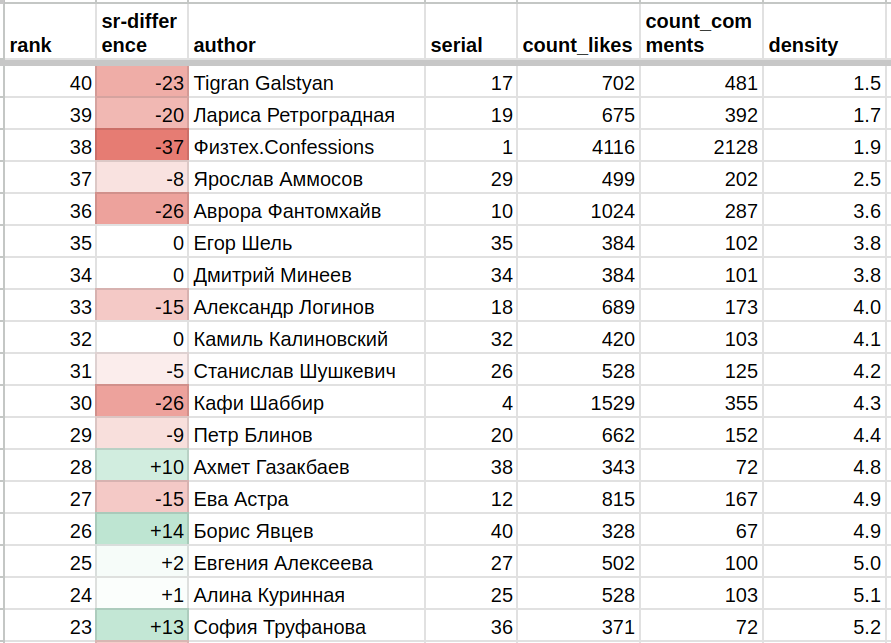
\includegraphics[width=0.75\textwidth]{table-reverse-density}
		\caption{Reverse density for the most based authors}
		\label{table-reverse-density}
	\end{figure}

	These authors are so \textbf{база} that people are probably afraid to like their comments, their comments are often misunderstood, if they carry a deeper meaning. Sometimes some of them are just trolling in massive amounts. There are a surprisingly large number of women in green (Евгения Алексеева, Алина Куринная, София Труфанова), these women have slightly higher densities than the average of the population. It is probably because the community of физтех-confessions and физтех is mostly male, and seeing female comments below the posts melts a man's heart.

	\begin{figure}[H]
		\centering
		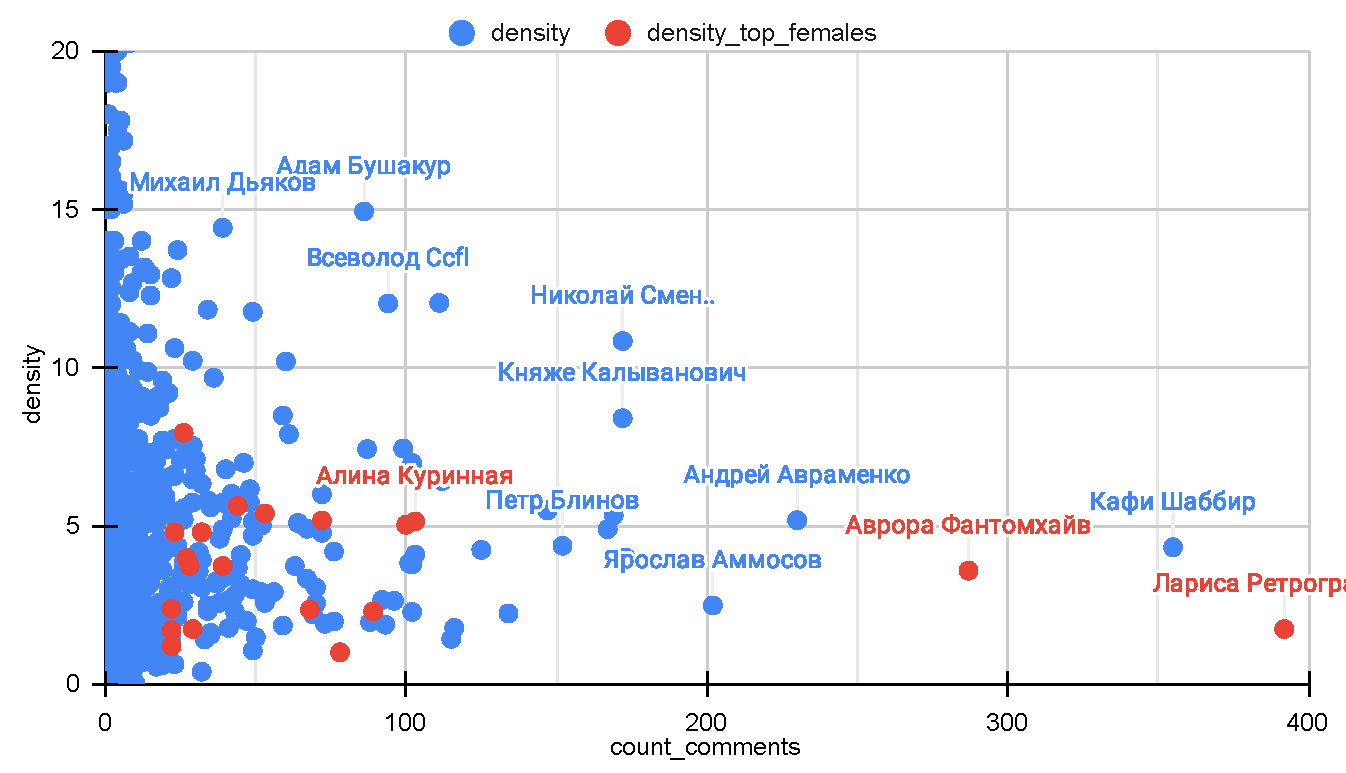
\includegraphics[width=1\textwidth]{fig-density-vs-count-comments}
		\caption{Density vs count\_comments, \cite{sheet-density-distribution}.}
		\label{fig-density-vs-count-comments}
	\end{figure}

	In figure \ref{fig-density-vs-count-comments}, all females who have commented more than 22 times are marked. It seems that they occupy a good position, often being on top of the blue blobs in that region. \textbf{Here the position of Адам Бушакур is absolutely legendary there is no one close to him in that region}.

\subsection{The best Female commentator}
	\begin{table}[H]
		\centering
		\caption{Top-12 female commentators based on count\_likes.}
		\label{table-female}
		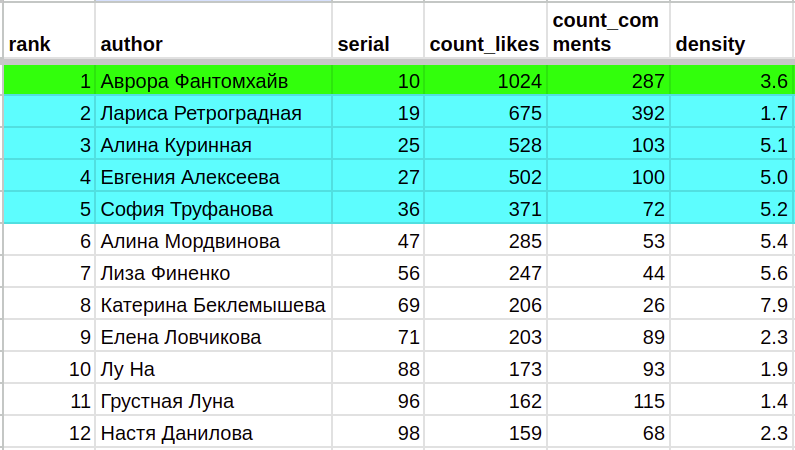
\includegraphics[width=0.7\textwidth]{table-female}
	\end{table}
	
\subsection{The most Productive commentator (h-index)}
	\begin{table}[H]
		\centering
		\caption{Top-20 most productive commentators.}
		\label{table-hindex}
		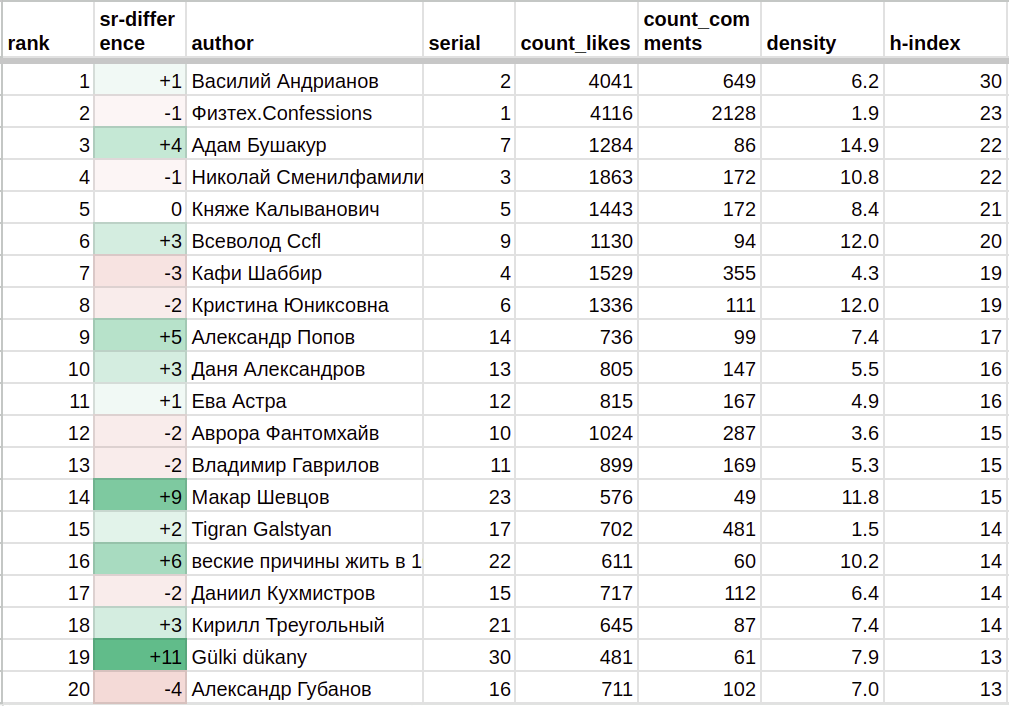
\includegraphics[width=0.9\textwidth]{table-hindex}
	\end{table}
	
	The density does not give us a full picture. Maybe an author writes a lot of compliments which decreases his density, or maybe he started out bad but now is doing good. Hence we judge them by the h-index \cite{wikipedia-hindex}.
	
	\newpage
	\vspace*{\fill}
	\begin{figure}[H]
		\centering
		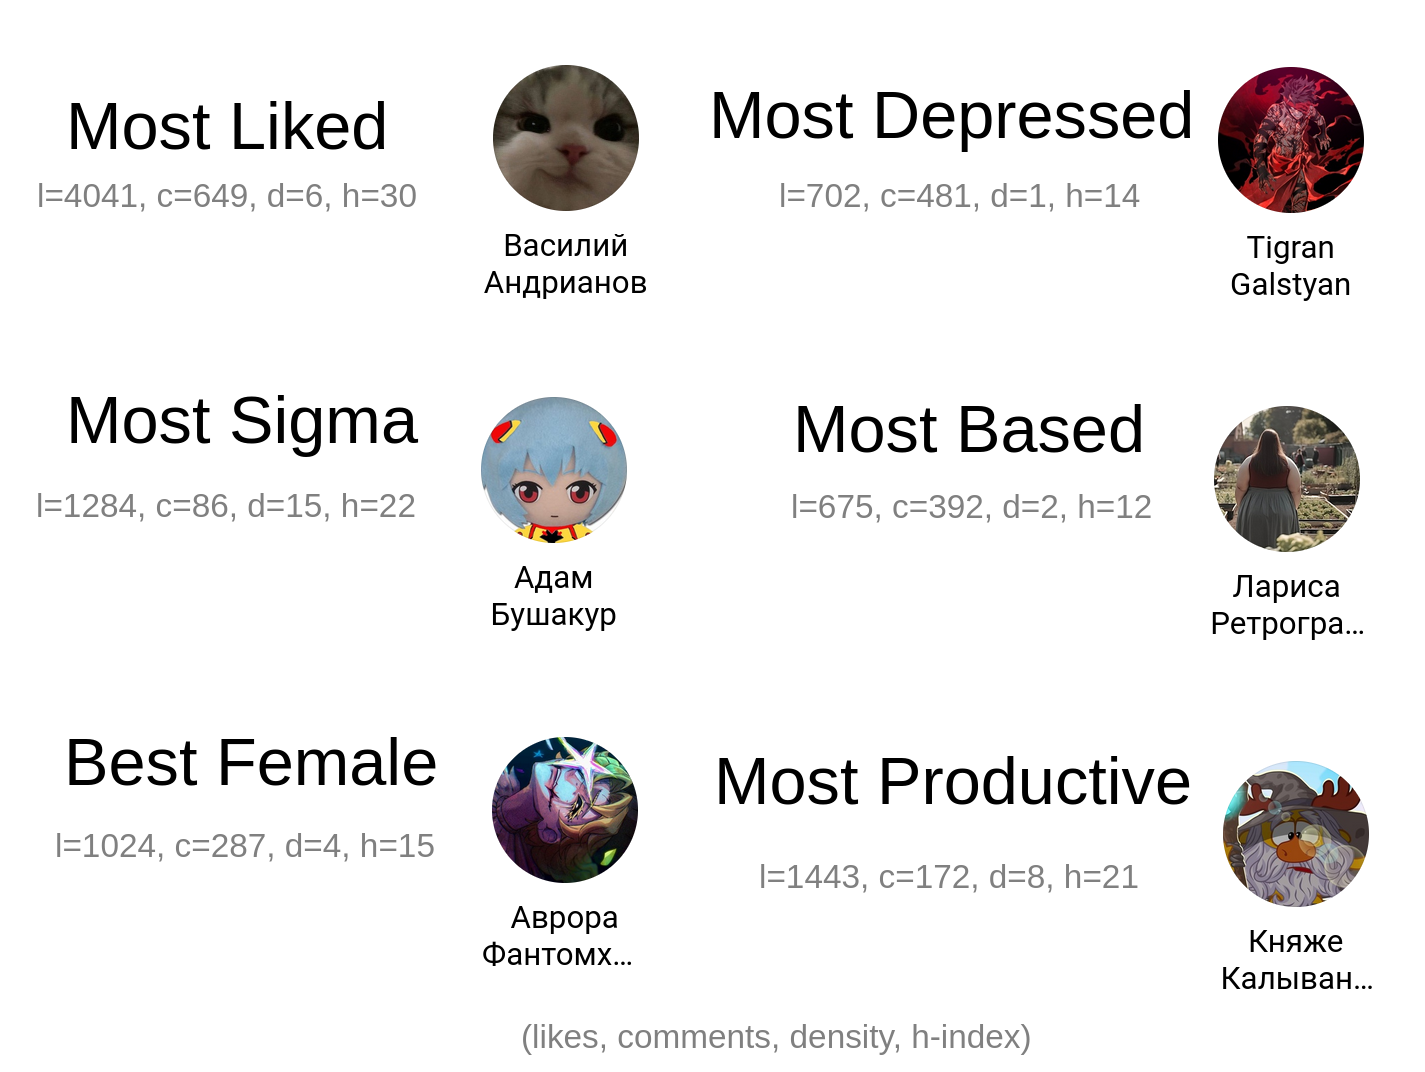
\includegraphics[width=\textwidth]{fig-authors-summary-pic}
		\caption{Top Commentators}
		\label{fig-authors-summary-pic}
	\end{figure}
	\vfill
	
\newpage
\section{Posts}
	\begin{figure}[H]
		\centering
		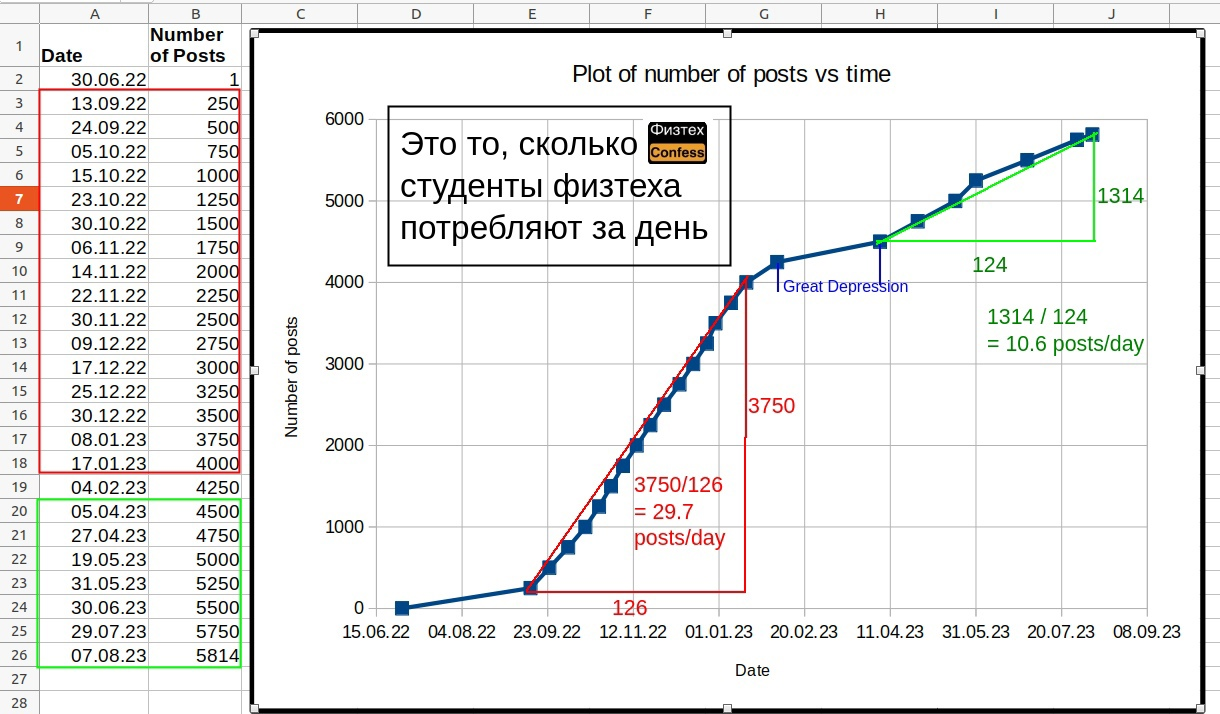
\includegraphics[width=0.8\textwidth]{fig-old-count-post-time}
		\caption{Statistics of number of posts over time, published in August 2023 in \#5818 \cite{vk-link-old-stats}}
		\label{fig-old-count-post-time}
	\end{figure}
	In figure \ref{fig-old-count-post-time}, for the first time in our life could see that, just like there are debt and credit cycles in the economy of a country, there are periods of less productivity of the writers and admins. Over here we see only one depression. Was it really the great depression? Did we have such a long depression again? Do these patterns of productivity and depressions happen over and over again? To answer this question we need to zoom out further out of this graph.

	\begin{figure}[H]
		\centering
		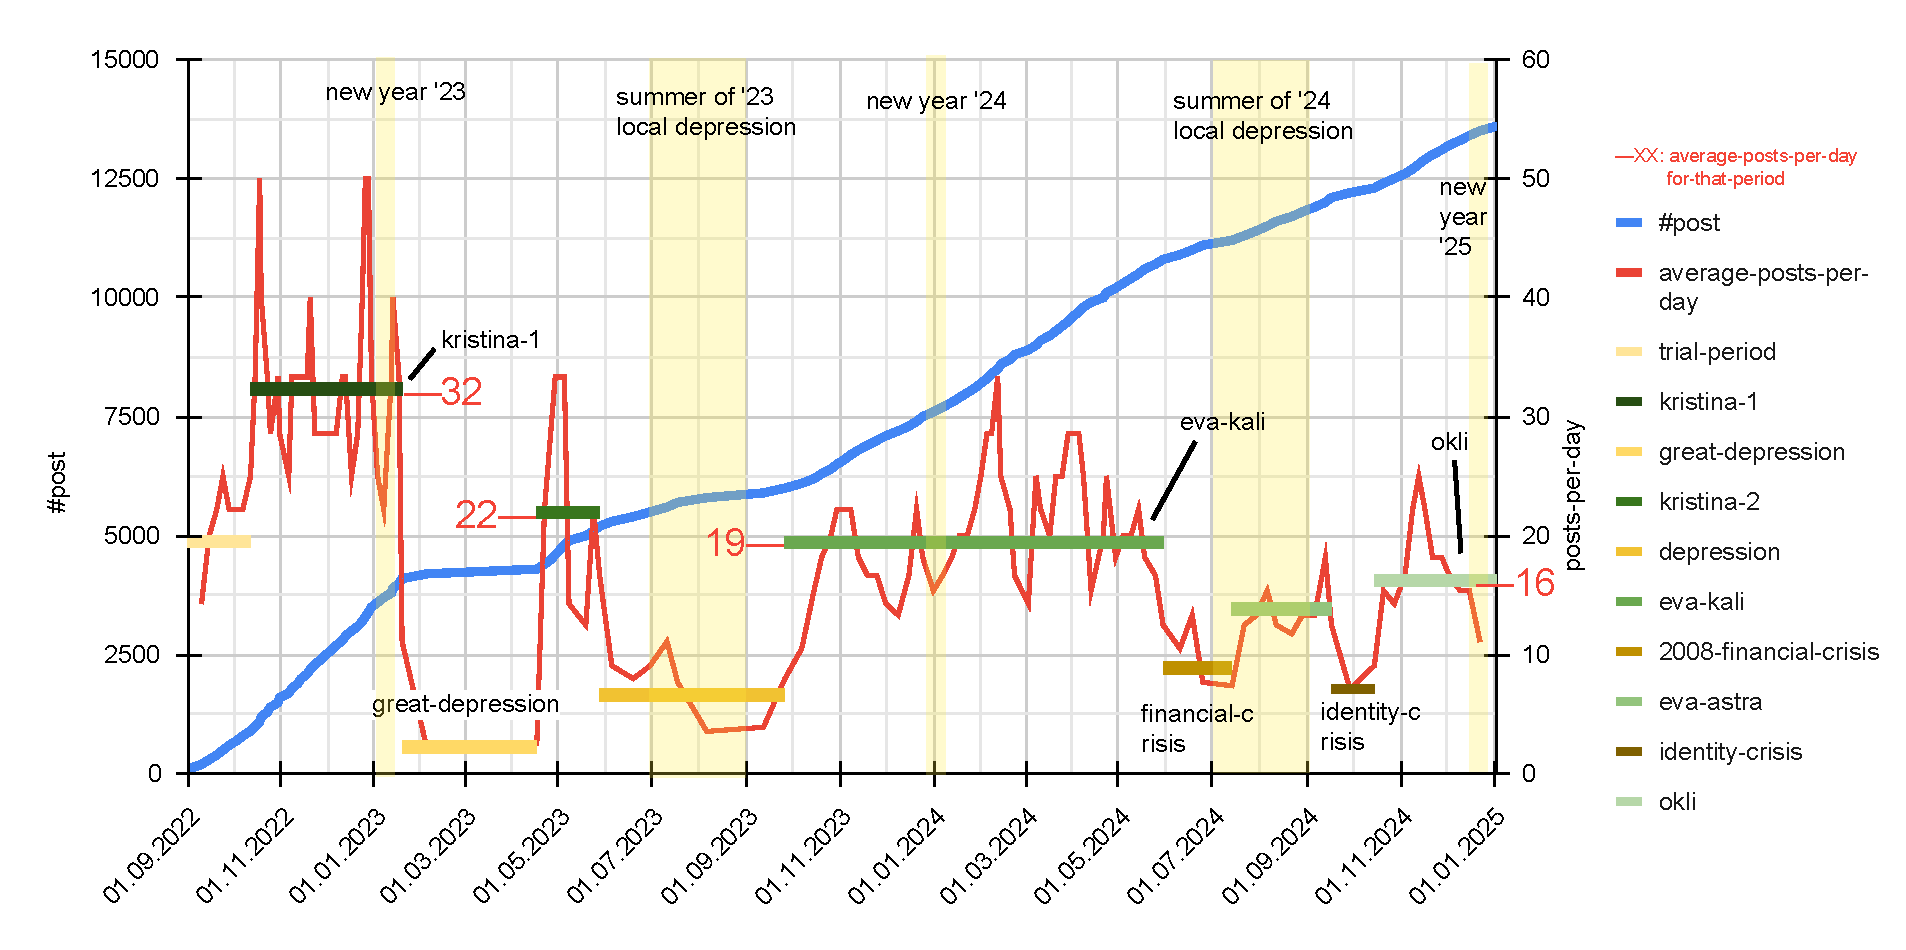
\includegraphics[width=1\textwidth]{fig-post-n-vs-time}
		\caption{Number of post published over time, and number of posts published per day for various periods of time \cite{sheet-post-vs-time}. This data was collected separately and the period is longer.}
		\label{fig-post-n-vs-time}
	\end{figure}
	
	In figure \ref{fig-post-n-vs-time}, we are looking at the whole history of confessions. The 100th post was published on 01.09.2022 and the 13600th post on 03.01.2025. That is 13501 posts published over 856 days, or \textbf{\num{15.7} posts per day}. The average number of likes per post from June 2023 to December 2024 is \num{22.4}. The activity starts slowly decreasing during examination sessions and significantly drops during vacations.
	
	\begin{enumerate}
		\item \textbf{trial-period} (01.09.2022 -- 15.10.2022): confessions was still being popularized. The number of posts per day (\num{20}) is very high compared to the less number of writers, which is strangely even higher than the current average posts per day under the reign of \textbf{Окли Сириус}, \num{16} posts per day.
	
		\item \textbf{kristina-1} (15.10.2022 -- 15.01.2023): the highest number of posts per day, slightly lower likes per post. Only written text was allowed, polls and pictures were mostly approved only on Sunday. The writers dumped a lot of trash and most content was published with little or less filtering. Kristina overworked during this period. (In sense of economics, a lot of growth was created by borrowing credits. Now each unit of credit created produces the same unit of debt, which needs to be paid in the future).
	
		\item \textbf{The great-depression} (15.01.2023 -- 15.04.2023): overworked Kristina was overwhelmed and needed to rest. This rest (depressed, gloomy sadness) period was a long 3 months. (It was time to pay back the large sum of debt accumulated that had been accumulated, the larger the debt -- the larger the crisis, or if the crisis is big enough can be called a depression).
		
		\item \textbf{kristina-2} (15.04.2023 -- 05.06.2023): a short active period, ended with the famous мама-таракан videos.
		
		\item \textbf{depression} (05.06.2023 -- 15.09.2023): a long general depression due to summer, a new admin was looked for during this period.
		
		\item \textbf{eva-kali} (15.09.2023 -- 15.06.2024): 9 months long, making it the longest period in the history, with a massive average of 19 posts per day. Here we see a sharp local drop during the new year of 2024. Eva kali was probably helped by Kristina. Jamclub was labeled as schizophrenia and much of it was banned. And most of what made through was on Sundays (aka день-говна).
		
		\item \textbf{astra-crises} (15.06.2023 -- 15.10.2024): there were enough posts per day to not designate them as depressions, but they were certainly crises. \textbf{2008-financial-crisis} began due to the start of exams in June, and in the middle of the summer eva, returned with a new name \textbf{eva-astra}, but kristina had probably quit by this time, but never the less there is a local peak. The overall activity during this period was much lower than any active periods. It ended with an \textbf{identity-crisis} when eva decided that she would need to prepare for ГОС, no one knew who the next admin would be, the new admin was selected in the public group chat.
		
		\item \textbf{okli} (15.10.2024 -- present): on 13.10.2024 around the post of \#12400, it was announced that \textbf{Окли Сириус} would be the new admin \cite{vk-announcement-of-okli}. This period saw a large increase in the number of picture based memes. Jamclub was given a new level of freedom.
	\end{enumerate}
	
	\begin{figure}[H]
		\centering
		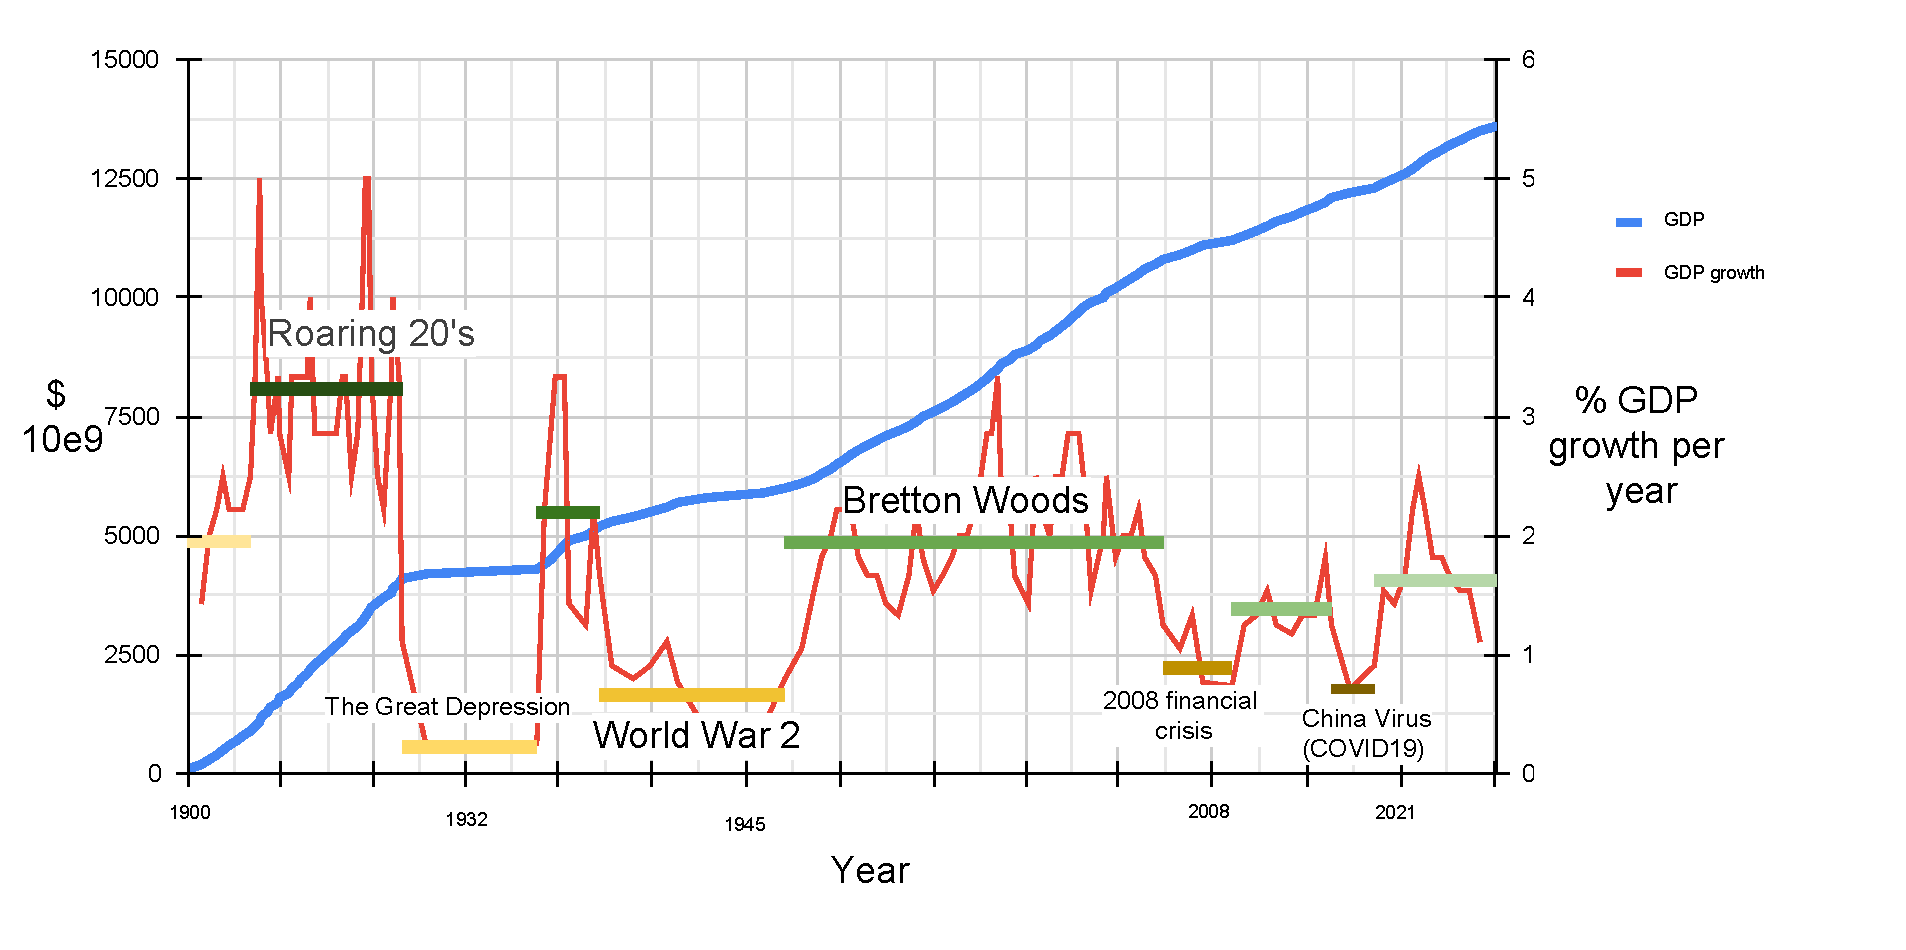
\includegraphics[width=1\textwidth]{fig-post-n-vs-time-joke}
		\caption{Marking periods in USA's econimic history on figure \ref{fig-post-n-vs-time}. This is the source for naming many of the periods.}
		\label{fig-post-n-vs-time-joke}
	\end{figure}
	
	
	\begin{figure}[H]
		\centering
		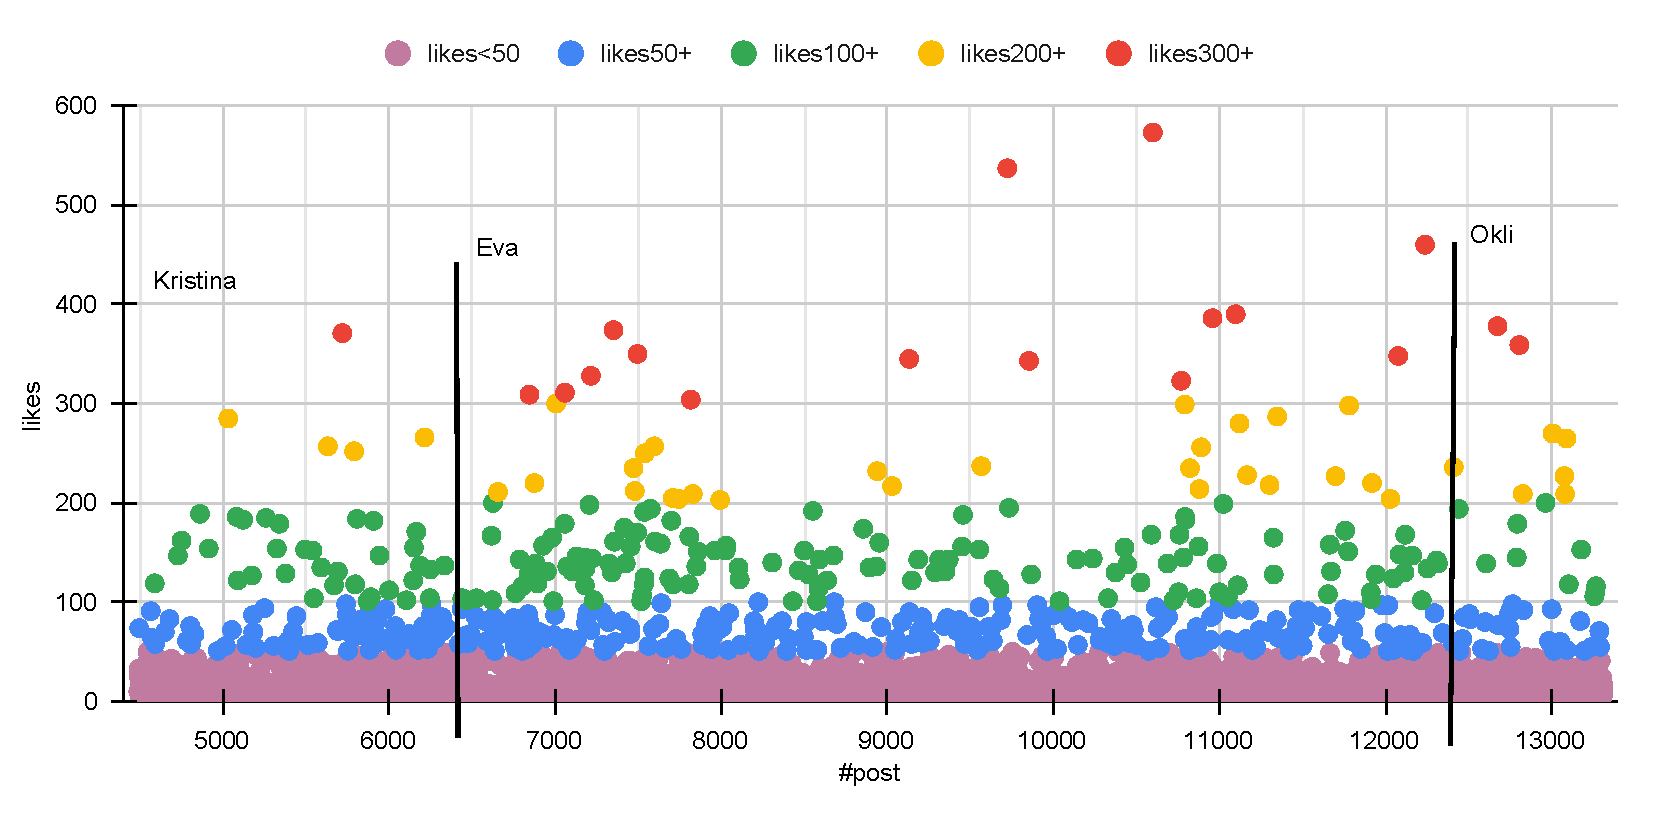
\includegraphics[width=1\textwidth]{fig-likes-mega-likes-vs-post-n}
		\caption{Likes by categories distiributed over hashtag-numbers of posts.}
		\label{fig-likes-mega-likes-vs-post-n}
	\end{figure}
	
	\begin{figure}[H]
		\centering
		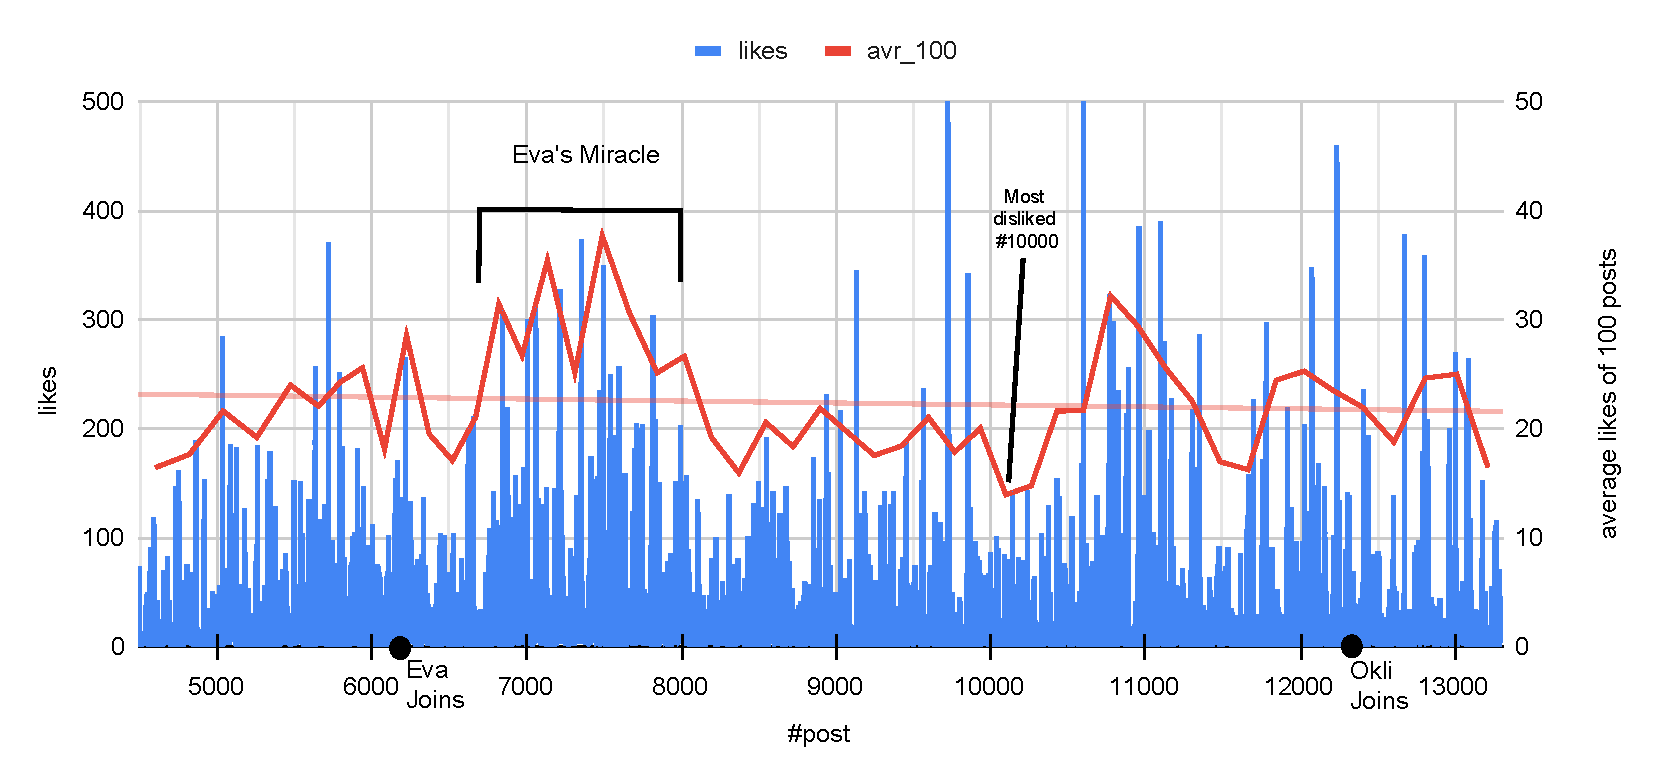
\includegraphics[width=1\textwidth]{fig-likes-vs-post-moving-average}
		\caption{Likes vs hashtag-number of posts, and (avr\_100) the average number of likes of surrounding 100 posts.}
		\label{fig-likes-vs-post-moving-average}
	\end{figure}
	
	The average number of likes per post very slightly decreased compared to the average, and significantly decreased compared to the period known as Eva's Miracle, where the number of posts and the likes per post was both high. The number of subscribers have steadily increased by a large margin over the year. However when we look at the trend-line of number of likes per post over time, the trend-line very slightly slopes downwards.
	
	\begin{figure}[H]
		\centering
		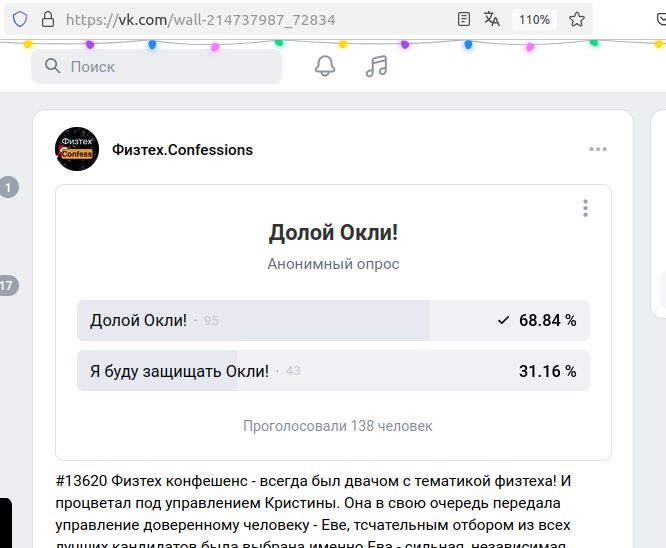
\includegraphics[width=0.7\textwidth]{fig-poll-for-okli-removal}
		\caption{Poll for removal of \textbf{Окли Сириус}, \#13620 \cite{vk-link-poll-removal-of-okli}.}
		\label{fig-poll-for-okli-removal}
	\end{figure}
	
	\textbf{Окли Сириус} claims that his method of [данные удалены] censorship is correct and is helping the community, because he sees positive statistics. This is a contradiction to the poll in figure \ref{fig-poll-for-okli-removal} where 65\% voters demand her removal. Many active writers and have stopped writing due to dissatisfaction with \textbf{Окли Сириус}'s policy of censorship.
		
	\begin{figure}[H]
		\centering
		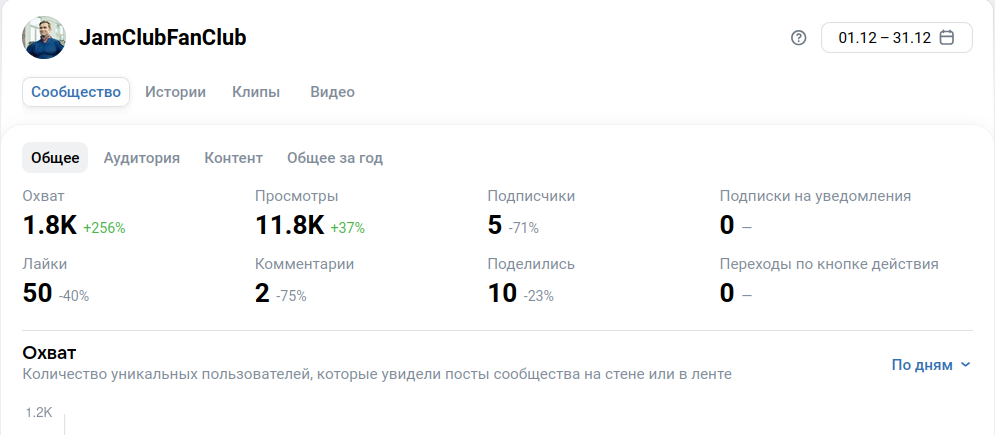
\includegraphics[width=1\textwidth]{fig-example-of-stats-vk}
		\caption{Example of community statistics, which most of the time shows positive results when the admins are sure they have not posted much.}
		\label{fig-example-of-stats-vk}
	\end{figure}
	
	\textbf{Окли Сириус} probably only looks at vk community page activity statistics, for example figure \ref{fig-example-of-stats-vk}. The vk community statics of физтех-confessions most probably shows that the activity is on the rise. 
	
	For example, the activity during the last month is higher than during the last 6 months. But this is misleading statistic. The activity during the last month will certainly be higher than during the last 6 months, because during the last 6 months, there were crisis periods, where there was no active admin.
	
	We can see in figure \ref{fig-post-n-vs-time} that financial and identity crises happeded (01.07.2024 - 01.10.2024). Also it is possible, vk probably chooses the reference points in such a way, that the initial points are located at the worst periods, thus maximizing the possibility of obtaining positive statistics. Vk does not care about the truth, it just wants to encourage people to use vk more and more. That is one reason why they do not have the dislike button.
				
	\textbf{Окли Сириус} and \textbf{Аврора Фантомхайв} claim that the activity under \textbf{Окли Сириус}'s reign has increased, they also claim that they can proof through statistics. \textbf{Мартин Рольгейз}, \textbf{Андрей Щапин} and \textbf{Даниил Городецкий}, have repeatedly requested \textbf{Окли Сириус} and \textbf{Аврора Фантомхайв} for the statistics (04.01.2024 - 06.01.2024), but their requests were ignored. Let us look at the most liked posts for May 2023 -- December 2024:
	
	\newpage	
	\vspace*{\fill}
	\begin{figure}[H]
		\centering
		
\includegraphics[width=0.9\textwidth]{fig-top-posts-10}
		\caption{Most liked post, at number-10}
		\label{fig-top-posts-10}
	\end{figure}
	\vfill
	
	\newpage	
	\vspace*{\fill}
	\begin{figure}[H]
		\centering
		
\includegraphics[width=0.9\textwidth]{fig-top-posts-9}
		\caption{Most liked post, at number-9}
		\label{fig-top-posts-9}
	\end{figure}
	\vfill
	
	\newpage	
	\vspace*{\fill}
	\begin{figure}[H]
		\centering
		
\includegraphics[width=0.9\textwidth]{fig-top-posts-8}
		\caption{Most liked post, at number-8}
		\label{fig-top-posts-8}
	\end{figure}	
	\vfill
	\begin{figure}[H]
		\centering
		
\includegraphics[width=0.9\textwidth]{fig-top-posts-7}
		\caption{Most liked post, at number-7}
		\label{fig-top-posts-7}
	\end{figure}
	\vfill
	
	\newpage	
	\vspace*{\fill}
	\begin{figure}[H]
		\centering
		
\includegraphics[width=0.9\textwidth]{fig-top-posts-6}
		\caption{Most liked post, at number-6}
		\label{fig-top-posts-6}
	\end{figure}
	\vfill
	
	\newpage	
	\vspace*{\fill}
	\begin{figure}[H]
		\centering
		
\includegraphics[width=0.9\textwidth]{fig-top-posts-5}
		\caption{Most liked post, at number-5}
		\label{fig-top-posts-5}
	\end{figure}
	\vfill
	
	\newpage	
	\vspace*{\fill}
	\begin{figure}[H]
		\centering
		
\includegraphics[width=0.9\textwidth]{fig-top-posts-4}
		\caption{Most liked post, at number-4}
		\label{fig-top-posts-4}
	\end{figure}
	\vfill
	
	\newpage	
	\vspace*{\fill}
	\begin{figure}[H]
		\centering
		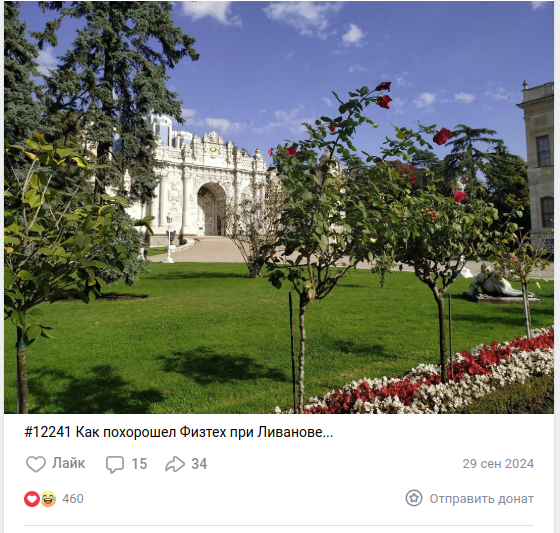
\includegraphics[width=0.9\textwidth]{fig-top-posts-3}
		\caption{Most liked post, at number-3}
		\label{fig-top-posts-3}
	\end{figure}
	\vfill
	
	\newpage		
	\vspace*{\fill}
	\begin{figure}[H]
		\centering
		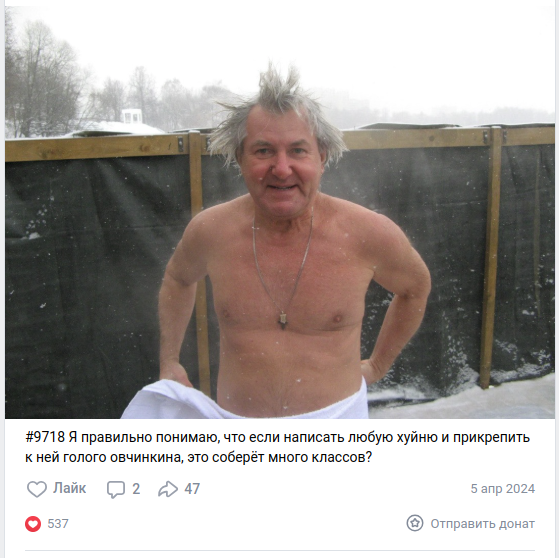
\includegraphics[width=0.9\textwidth]{fig-top-posts-2}
		\caption{Most liked post, at number-2}
		\label{fig-top-posts-2}
	\end{figure}
	\vfill
	
	\newpage	
	\vspace*{\fill}
	\begin{figure}[H]
		\centering
		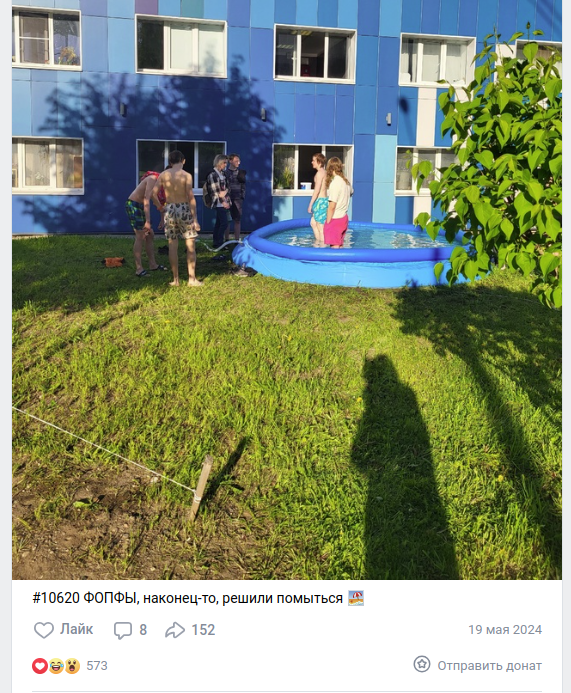
\includegraphics[width=0.9\textwidth]{fig-top-posts-1}
		\caption{Most liked posts at number-1}
		\label{fig-top-posts-1}
	\end{figure}
	\vfill
\newpage
\section{Conclusions}
	\begin{enumerate}
		\item There are a huge number of authors who have commented less than 20 times in their life, since \num{500} out of \num{1778} authors account for \num{93}\% of all likes on comments.
		
		\item The top 40 authors account for half the comment activity.
		
		\item The average number of posts per day under the reign of \textbf{Окли Сириус} is \num{16}, which is the lowest compared to \textbf{kristina-1}, \textbf{kristina-2}, and \textbf{eva-kali}, which had average post per day of: 32, 22, and 19 respectively. Even tough the number of subscribers increased, the number of writers decreased due illogical censorships of [данные удалены].
		
		\item Even tough the number of memes increased under \textbf{Окли Сириус}, and memes get significantly higher number of likes, the average likes per post did not change from the average. And is significantly lower than the Eva's Miracle period in figure \ref{fig-likes-vs-post-moving-average}.
		
		\item Vk-statistics can be misleading in the case of физтех-confessions, as we do not have continuous posts over the year and there are significant periods of depressions. Therefore any active period will look better than the average. So for correct conclusions, data such as posts and likes over time needs to be manually obtained and analyzed period by period. And only active periods needs to be compared with one another.
		
		\item The activity starts slowly decreasing during examination sessions and significantly drops during vacations.
		
	\end{enumerate}
	
\newpage
\bibliographystyle{plain.bst}
\bibliography{reference}
\end{document}
